\section{はじめに}

当サークルのマスコットキャラクターであるKaiRA君を動かして愛でてみたい、というのがこのプロジェクトを製作した動機です。当プロジェクトでは、ユーザーが自然言語による命令を入力すると、KaiRA君がそれに従って動いてくれます。命令と動きによる応答の関係を通じて、時には命令にうまく従ってくれないことも含め、KaiRA君との不思議な交流が楽しめます。

\begin{figure}[htbp]
    \centering
    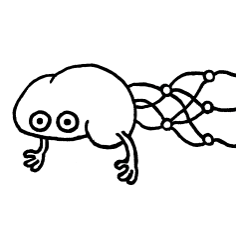
\includegraphics[width=0.5\textwidth]{moving-kaira-kun/fig/kaira_kun.png}
    \caption{当プロジェクトで使用したKaiRA君のイラスト}
    \label{fig:kaira_kun}
\end{figure}

\section{モーションの生成}

KaiRA君のモーションを自然言語から生成するために、当プロジェクトではHuman Motion Diffusion Model\cite{tevet2022humanmotiondiffusionmodel}を用いています。テキストからモーションを生成するモデルはこれ以外にも、MotionGPT\cite{jiang2023motiongpthumanmotionforeign}等が挙げられます。しかし、生成されるモーションの質に大きな差が見られなかったので、生成速度の観点からこの手法を選択しました。Human Motion Diffusion Modelは、ノイズを50ステップという少ないステップ数で取り除いても十分な質のモーションを生成できます。

Human Motion Diffusion Modelはその名の通り、基本的な生成の仕組みは拡散モデルに基づいています。Transformerのエンコーダ部分を用いて、各時刻における関節の位置や回転が予測されています。ただし、学習に用いられる損失関数には工夫が施されていて、通常の拡散モデルによる手法のものとは異なります。通常はある時刻で与えたノイズと、それを予測したノイズとの間で損失を取りますが、この手法ではノイズが加えられる前のものと、ある時刻でノイズが除去された後のものとの間で損失を取っています。これに、各関節の位置や速度の予測と正解の差を考慮した損失を組み合わせたものを用いて、学習を行っています。

\begin{figure}[htbp]
    \centering
    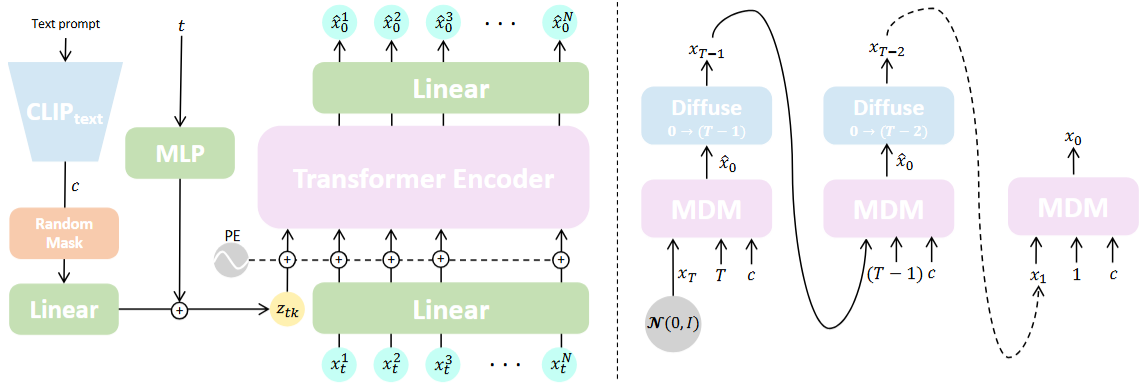
\includegraphics[width=0.8\textwidth]{moving-kaira-kun/fig/hdm_overview.png}
    \caption{Human Motion Diffusion Modelの全体像}
    \label{fig:hdm_overview}
\end{figure}

Human Motion Diffusion Modelで生成されたモーションは、NumPy配列として出力されます。当プロジェクトでは、出力されたNumPy配列をBVHファイルに変換したものをAnimated Drawingsに入力しています。

\section{アニメーションの生成}

生成されたモーションに従ってKaiRA君を動かすために、当プロジェクトではAnimated Drawings\cite{smith2023methodanimatingchildrensdrawings}を用いています。実のところ、当初は2Dのアニメーションではなく、KaiRA君の画像から生成した3Dモデルを用いるつもりでした。しかし、LRM\cite{hong2024lrmlargereconstructionmodel}やDreamGaussian\cite{tang2024dreamgaussiangenerativegaussiansplatting}等の手法を試したものの、平面的な1枚のイラストを3Dにうまく変換することはできませんでした。そのような経緯で、3Dモデルを生成することは一旦諦め、KaiRA君を2Dのイラストのまま動かすことにしました。

Animated Drawingsは、キャラクターの関節の位置を1枚の画像から推定し、それを基づいてアニメーションを生成することが可能です。しかし、学習に用いられたイラストは人の形をしたものが多いため、KaiRA君に対して自動で関節を割り当ててもうまく機能しません。また、KaiRA君は人間のような下半身を持たないため、生成された人間のモーションをそのまま適用すると、胴体がねじれる等の不都合が生じます。そこで当プロジェクトでは下図のように、腕の動きを反映させることを重視し、下半身の関節については画像の下端に配置することで、その影響をなるべく排除しています。

\begin{figure}[htbp]
    \centering
    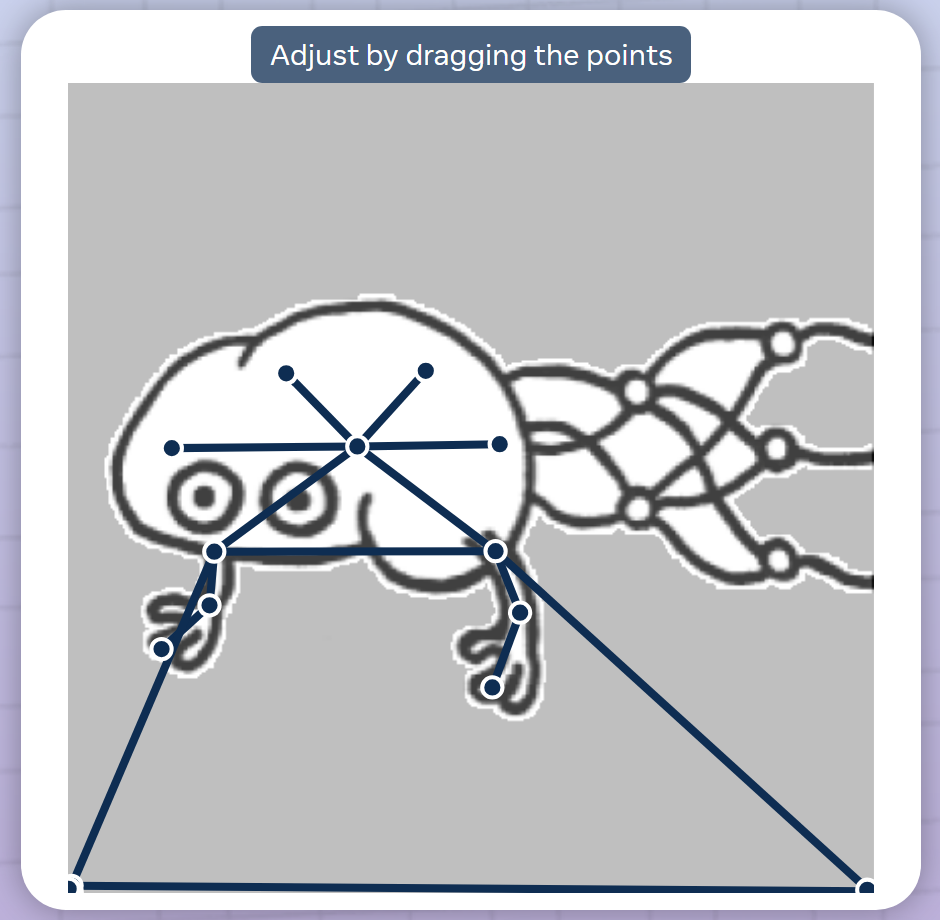
\includegraphics[width=0.5\textwidth]{moving-kaira-kun/fig/kaira_kun_animated_drawings.png}
    \caption{KaiRA君の関節の配置の設定}
    \label{fig:kaira_kun_animated}
\end{figure}

Animated DrawingsはBVHファイルにより、アニメーションの動きを指定することができます。このとき入力されるモーションは3Dですが、これを平面に投影することでキャラクターの関節と対応させています。ただし、BVHファイルの関節と、キャラクターの関節との対応関係は手動で設定する必要があります。

\begin{figure}[htbp]
    \centering
    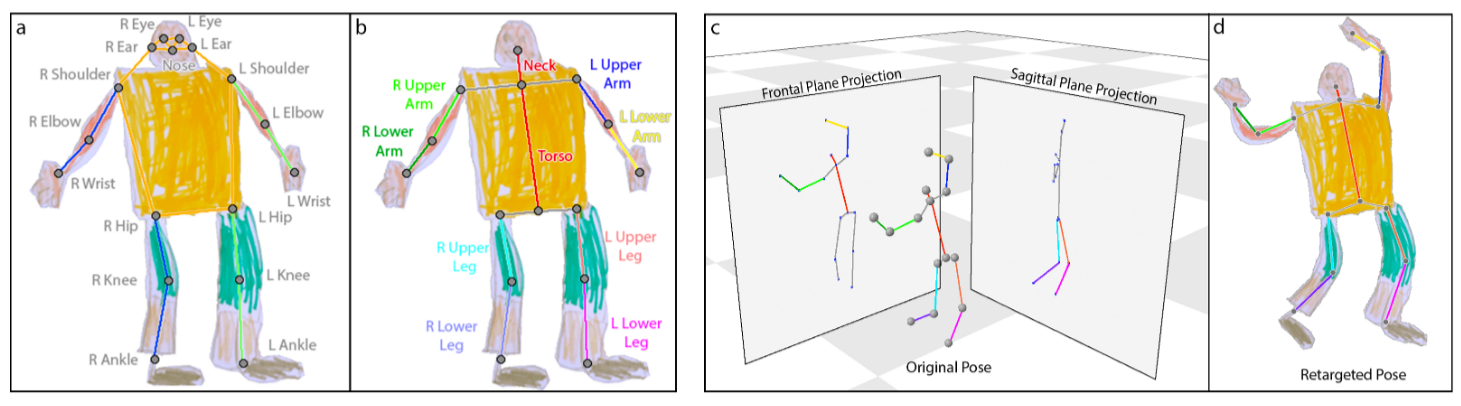
\includegraphics[width=0.8\textwidth]{moving-kaira-kun/fig/animated_drawings.png}
    \caption{Animated Drawingsの全体像}
    \label{fig:animated_drawings}
\end{figure}

Animated Drawingsの手法の詳細には立ち入りませんが、これをHuman Motion Diffusion Modelと組み合わせることで、自然言語の命令によりKaiRA君をアニメーションで動かすことが可能になります。

\section{おわりに}

現在のAIはすでに高度な言語処理能力を持つようになりましたが、現実の人間による言語活動は純粋な言語でのみ構成されるものではなく、身体的な要素が多大に含まれています。その意味では、言語と身体を繋ぐ道具として、テキストからモーションを生成する手法は想像以上に重要かもしれません。当プロジェクトでは人間が入力したテキストを用いてモーションを生成していますが、AIが自ら適切なモーションを選択し生成できるようになれば、人間とAIのコミュニケーションはより豊かなものになり得ると思います。
